\documentclass{summarysheet}

\begin{document}


\maketitle{8}{The Magnetic Field}

\begin{multicols}{2}

\begin{topicbox}{Magnetic Field}

\noindent \emph{Moving charges} create magnetic fields.  For a single point charge, the magnetic field is given by the \emph{Biot-Savart law},
\begin{multicols}{2}
\begin{eqbox}
\vec{B} = \frac{\mu_0}{4\pi} \frac{q\vec{v} \times \hat{r}}{r^2},
\end{eqbox}
where $\mu_0 = 4\pi \times 10^{-7}$ Tm/A is the \emph{permeability constant}.
\begin{center}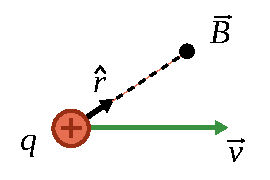
\includegraphics[scale=0.5]{fig_bs_point.pdf}\end{center}
\end{multicols}

\begin{multicols}{2}
For a current segment of length $d\vec{s}$, the Biot-Savart law is
\begin{eqbox}
\vec{B} = \frac{\mu_0}{4\pi} \frac{Id\vec{s} \times \hat{r}}{r^2}.
\end{eqbox}
\begin{center}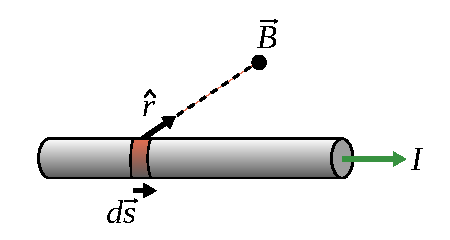
\includegraphics[scale=0.5]{fig_bs_wire.pdf}\end{center}
\end{multicols}

Some common fields are:
\begin{itemize}
\begin{multicols}{2}
\item A distance $r$ from long straight wire carrying current $I$
\[
B = \frac{\mu_0 I}{2\pi r}
\]
\begin{center}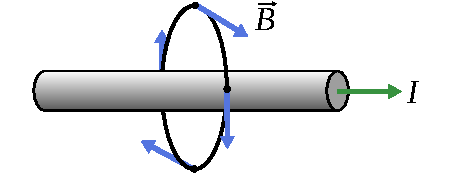
\includegraphics[scale=0.5]{fig_B_wire.pdf}\end{center}
\end{multicols}

\begin{multicols}{2}
\item At the centre of an $\theta$ radian arc of wire or radius $R$ and carrying current $I$
\[
B = \frac{\mu_0 I \theta}{4\pi R}
\]
\begin{center}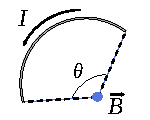
\includegraphics[scale=0.9]{fig_B_arc.pdf}\end{center}
\end{multicols}

\begin{multicols}{2}
\item At the centre of a loop of $N$ turns and radius $R$, carrying current $I$
\[
B = \frac{\mu_0 N I}{2R}
\]
\begin{center}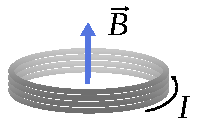
\includegraphics[scale=0.7]{fig_B_coil.pdf}\end{center}
\end{multicols}

\begin{multicols}{2}
\item Inside a solenoid of length $\ell$ and number of turns $N$, carrying current $I$
\[
B = \frac{\mu_0 N I}{\ell}
\]
\begin{center}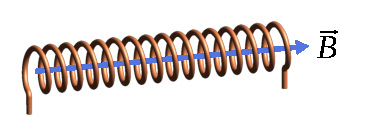
\includegraphics[scale=0.6]{fig_B_solenoid.pdf}\end{center}
\end{multicols}

\end{itemize}

\end{topicbox}



\begin{topicbox}{Amp\`ere's Law}

\noindent Amp\`ere's law states that the line integral of the magnetic field around a closed loop is proportional to the current passing through that loop:
\begin{eqbox}
\oint \vec{B} \cdot d\vec{s} = \mu_0 I_\text{through}.
\end{eqbox}
This is useful for highly symmetric current distributions.
\end{topicbox}


\begin{topicbox}{Magnetic Forces}

\noindent Magnetic fields exert a \emph{force} on \emph{moving charges}:
\begin{eqbox}
\vec{F}_\text{on $q$} = q \vec{v} \times \vec{B}.
\end{eqbox}

\noindent \textbf{Cyclotron Motion}

\noindent A charged particle moving perpendicular through a uniform magnetic field undergoes \emph{cyclotron motion}, with radius $r_\text{cyc}$ and frequency $f_\text{cyc}$ given by
\[
r_\text{cyc} = \frac{mv}{qB} \quad \text{and} \quad f_\text{cyc} = \frac{qB}{2\pi m}.
\]

\noindent \textbf{Force on a wire}

\noindent Magnetic fields also exert a force on \emph{current-carrying wires}:
\begin{eqbox}
\vec{F}_\text{wire} = I \vec{\ell} \times \vec{B},
\end{eqbox}
\noindent where $\ell$ points in the direction of the current.

\noindent \textbf{Force between wires}

\noindent Two parallel wires of current $I_1$ and $I_2$, of length $\ell$ and separated by a distance $d$, will therefore exert a force on each other (attractive for current in the same direction, repulsive for opposite currents), with magnitude
\[
F = \frac{\mu_0 \ell I_1 I_2}{2\pi d}.
\]

\end{topicbox}


\begin{topicbox}{Magnetic Dipoles}

\noindent A current loop of area $A$ is a magnetic dipole, with dipole moment
\begin{eqbox}
\vec{\mu} = (AI, \text{south to north pole}).
\end{eqbox}

\noindent The magnetic field on the axis far from the loop at distance $z$ is given by
\[
\vec{B}_\text{dipole} = \frac{\mu_0}{4\pi} \frac{2\vec{\mu}}{z^3}.
\]
A uniform magnetic field exerts no net force on the current loop, but will exert a torque
\[
\vec{\tau} = \vec{\mu} \times \vec{B},
\]
which tends to rotate the loop so that the dipole moment is aligned with the magnetic field.

\begin{center}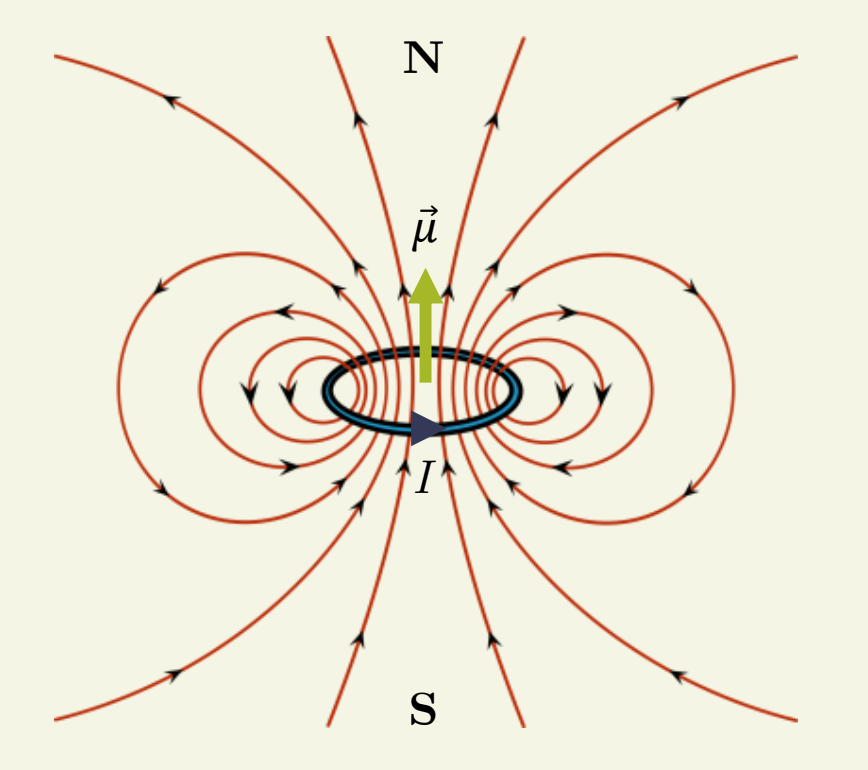
\includegraphics[scale=0.15]{fig_dipole.png}\end{center}

\end{topicbox}
\end{multicols}


\begin{topicbox}{Magnetism in Materials}

\begin{multicols}{2}
Atomic electrons in a material have a magnetic dipole moment due to a property called spin. In some materials, called ferromagnetic, these dipole moments can align to create a strong magnetic field. The image to the right shows the domain structure of a ferromagnet; within each
domain the dipole moments combine.

\begin{center}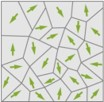
\includegraphics[scale=0.8]{fig_mag_domain.jpg}\end{center}
\end{multicols}
\end{topicbox}

\makebanner{Electricity and Magnetism}

\end{document}



